\documentclass[12pt]{article}
\usepackage[utf8]{inputenc}

\usepackage{lmodern}

\usepackage{enumitem}
\usepackage[margin=2cm]{geometry}

\usepackage{amsmath, amsfonts, amssymb}
\usepackage{graphicx}
%\usepackage{subfigure}
\usepackage{tikz}
\usepackage{pgfplots}
\usepackage{multicol}

\usepackage{comment}
\usepackage{url}
\usepackage{calc}
\usepackage{subcaption}
\usepackage[indent=0pt]{parskip}
\usepackage{animate}

\usepackage{array}
\usepackage{blkarray,booktabs, bigstrut}
\usepackage{bigints}

\pgfplotsset{compat=1.16}

% MATH commands
\newcommand{\ga}{\left\langle}
\newcommand{\da}{\right\rangle}
\newcommand{\oa}{\left\lbrace}
\newcommand{\fa}{\right\rbrace}
\newcommand{\oc}{\left[}
\newcommand{\fc}{\right]}
\newcommand{\op}{\left(}
\newcommand{\fp}{\right)}

\newcommand{\bi}{\mathbf{i}}
\newcommand{\bj}{\mathbf{j}}
\newcommand{\bk}{\mathbf{k}}
\newcommand{\bF}{\mathbf{F}}

\newcommand{\mR}{\mathbb{R}}

\newcommand{\ra}{\rightarrow}
\newcommand{\Ra}{\Rightarrow}

\newcommand{\sech}{\mathrm{sech}\,}
\newcommand{\csch}{\mathrm{csch}\,}
\newcommand{\curl}{\mathrm{curl}\,}
\newcommand{\dive}{\mathrm{div}\,}

\newcommand{\ve}{\varepsilon}
\newcommand{\spc}{\vspace*{0.5cm}}

\DeclareMathOperator{\Ran}{Ran}
\DeclareMathOperator{\Dom}{Dom}

\newcommand{\exo}[1]{\noindent\textcolor{red}{\fbox{\textbf{Problem {#1}}}\hrulefill}\\}
\newcommand{\qu}[4]{\noindent\textcolor{#4}{\fbox{\textbf{Section {#1} | Problem {#2}}} \hrulefill{{\fbox{\textbf{{#3} Points}}}}\\}}

\newcommand{\semester}{Spring 2023}

\newcommand{\CVup}{%

\begin{tikzpicture}
\draw[black, <->, >=latex] (-0.33, 0.5) .. controls (-0.125, 0) and (0.125, 0) .. (0.33, 0.5);
\end{tikzpicture}}

\newcommand{\CVupInc}{%
\begin{tikzpicture}
\draw[black, ->, >=latex] (0,0) .. controls (0.2, 0) and (0.4, 0.2) .. (0.5, 0.5);
\end{tikzpicture}}

\newcommand{\CVupDec}{%
\begin{tikzpicture}[rotate=270]
\draw[black, ->, >=latex] (0,0) .. controls (0.2, 0) and (0.4, 0.2) .. (0.5, 0.5);
\end{tikzpicture}}

\newcommand{\CVdown}{%
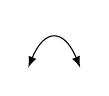
\begin{tikzpicture}
\draw[black, <->, >=latex] (-0.33, -0.5) .. controls (-0.125, 0) and (0.125, 0) .. (0.33, -0.5);
\end{tikzpicture}}

\newcommand{\CVdownInc}{%
\begin{tikzpicture}
\draw[black, ->, >=latex] (-0.5, -0.5) .. controls (-0.5, -0.3) and (-0.5, -0.1) .. (0,0);
\end{tikzpicture}}

\newcommand{\CVdownDec}{%
\begin{tikzpicture}[rotate=-90]
\draw[black, ->, >=latex] (-0.5, -0.5) .. controls (-0.5, -0.3) and (-0.5, -0.1) .. (0,0);
\end{tikzpicture}}

\begin{document}
	\noindent \hrulefill \\
	MATH-241 \hfill Pierre-Olivier Paris{\'e}\\
	Solutions Section 3-2 \hfill \semester \\\vspace*{-1cm}
	
	\noindent\hrulefill
	
	\spc
		
	\exo{12}
	\\
	Since $f$ is a polynomial, then it is continuous and differentiable on $[-2, 2]$. Therefore, the hypothesis of the MVP are satisfied. We want to find all solutions $c$ to
		\begin{align*}
		f' (c) = \frac{f (2) - f(-2)}{2 - (-2)} = \frac{f(2) - f(-2)}{4} .
		\end{align*}
	
	The derivative of $f$ is 
		\begin{align*}
		f'(x) = 3x^2 - 3 .
		\end{align*}
	Therefore, we look for numbers $c$ such that
		\begin{align*}
		3c^2 - 3 = \frac{4 - 0}{4} = 1 .
		\end{align*}
	So, $c$ should be a solution of
		\begin{align*}
		3c^2 = 4 \iff c = \pm \frac{2}{\sqrt{3}} .
		\end{align*}
	
	The numbers that satisfy the Mean Value Theorem are $c = -2/\sqrt{3}$ and $c = 2/\sqrt{3}$. 
	
	\spc
	
	\exo{20}
	\\
	The function $f (x) = 2x - 1 - \sin x$ is continuous. It is also differentiable at every point. We can apply the IVT and the MVT.
	
	We first use the IVT to show that there is at least one root. We see that $f(0) = -1 < 0$ and $f(\pi ) = 2\pi - 1 > 0$. So, letting $N = 0$ in the IVT, we conclude that there is a number $c$ between $0$ and $\pi$ such that $f(c) = 0$. 
	
	We secondly use the MVT to show that there is only one root. The derivative of $f(x)$ is $f'(x) = 2 - \cos x$. If there were two roots to the equation $f(x) = 0$, call them $c_1$ and $c_2$, then $f(c_1) = f(c_2) = 0$ and from the MVT we conclude that there is a $\tilde{c}$ between $c_1$ and $c_2$ such that $f'(\tilde{c}) = 0$. But $f'(x) = 2 - \cos x > 0$ for any number $x$ because $-1 \leq \cos x \leq 1$. This is a contradiction. So, there must be only one root to the equation $f(x) = 0$.
	
	\spc
	
	\exo{30}
	\\
	Fix $b > 0$. An odd function on $[-b, b]$ means that $f(-x) = -f(x)$ for any $x$ in $[-b, b]$.
	
	Since $f$ is differentiable, from the Mean Value Theorem, there exists a $c$ in $(-b, b)$ such that
		\begin{align*}
		f'(c) = \frac{f(b) - f(-b)}{2b} .
		\end{align*}
	However, $f(-b) = -f(b)$ and therefore
		\begin{align*}
		 \frac{f(b) - f(-b)}{2b} = \frac{f(b) + f(b)}{2b} = \frac{f(b)}{b} .
		\end{align*}
	So, combining everything together, there exists a $c$ in $(-b, b)$ such that 
		\begin{align*}
		f'(c) = \frac{f(b)}{b} .
		\end{align*}
	This completes the proof.
	
	
	
\end{document}